\section{Introduction}
We would like to start presenting the motivation for this thesis, and the concepts used throughout, but first we would like to include the purpose of the thesis. In our thesis contract we have the following description of the purpose of the thesis in danish:\\\\
The purpose with the thesis is to learn how neural networks is based theoretically, to learn how they can be applied to solve specific tasks, in this case to predict proteins' properties based on their composition of amino acids, and a basic understanding of those. \\\\
We expect the thesis to have the following parts:\\
- A rudimentary implementation of a neural network without use of newer tools, with the motivation to be able to explain the theoretical background for it.\\
- A real implementation of a artificial neural network based on established frameworks, as Pytorch, with the motivation to be able to predict proteins secondary structures, based on a sequence of amino acids. \\
- A similar implementation with the motivation of being able to predict Solvent Accessible Surface Area based on amino acid sequences. \\
- A comparison of result from the two above mentioned models, contrasted with a model that use multi-tasking to predict both of those properties.\\ 

Using this description as a guide through our work, we started with a look at the rudementary implentation of a neural network. As a starting point for this, we were given a jupyter-notebook with some introductory explanations and excercises to do.
It can be found at \href{https://github.com/dennybritz/nn-from-scratch/blob/master/nn-from-scratch.ipynb}{Github}.
Besides doing the excercises and playing with the code to get a better understanding of the methods and concepts, we afterwords implemented the same neural network using pytorch. 
This gave us a basis understanding of where to start coding our real neural networks. As it was used as a practice excersise for us to get started and giving a base understanding, we have decided not to include the code or excersises in the thesis, as it wouldn't add anyting relevant, though the understanding gained is part of our explaination in the method section of the thesis. Before going there though, we would like to finish introducing the background for this thesis.

\subsection{Motivation}
In computer science today, one of the areas that are the most in the public eye and covered by media and politicians alike is the area of Artificial Intelligence. Within this area concepts like deep learning, machine learning and neural networks are showing up repeatedly as buzzwords and central areas for future research and use.\\
It is in this context the motivation to have neural networks as a topic for this thesis has it's origins. This thesis' purpose is threefold. The first is to give an introductory understanding of the topic of machine learning and more specifically neural networks. This includes a basic understanding of the theoretical basis of neural networks. \\
Secondly the purpose is to widen this understanding of neural networks by implementing one to handle a specific task. This task is to predict secondary structure of proteins based on their amino acid composition. Lastly the purpose is to give an rudimentary understanding of of those proteins to give context to the use of the neural network.\\
The motivation for choosing protein secondary structure prediction for the neural networks also has several reasons. 
The textbook example when learning about neural networks and implementing them is to identify a handwritten number between 0 and 9. This neural network is often trained on the MNIST dataset of handwritten numbers. \\
Since many people has done this, and the application and importance of this in the real world is limited there would be very little content to this thesis if that had been the context. We will come back to the MNIST dataset of numbers though, to explain some of the basics of neural networks. Protein secondary structure prediction on the other hand has more real world applications and are an important branch of bioinformatics, and is used in both medicine and biotechnology. Since it is an important topic with real world use, it is an area that is still under research to improve the prediction accuracy. As such it gives a current and relevant context for this thesis as an interesting introduction to neural networks and their application.   


\subsection{Proteins}
Proteins are large bio molecules that has a wide range of functions in organisms. Those functions includes giving structure to cells, being part of DNA replication and responding to stimuli. KILDEKILDEKILDE!!. They consist of a chain of amino acids, where it is the sequence of the amino acids that determine the protein. The linear sequence of amino acids in a protein is also known as a proteins primary structure. 

\subsubsection{Secondary Structures}
The secondary structures are the three dimensional forms a protein can take in a local segment and are largely determined by it's primary structure. Among the many reasons for predicting the secondary structure, using it as a stepping stone for trying to find the three-dimensional structure of a protein, which is normally difficult to assess. The secondary structure itself is the three-dimensional form of local segments of the protein \citep[p.~2]{qi-et-al-2012}.
The secondary structure is divided into groups of either 3 or 8 types of structure, named Q3 and Q8 \citep{zhou-and-troyanskaya-2014}. 
Using the DSSP alphabet \citep{kabsch-and-sander-1983} 
for giving the groups letters, the categories of Q8 are as shown in the Q8 table \citep{qi-et-al-2012}.
\begin{table}[H]
\caption{Q8 structure overview}
\centering
\begin{tabular}{l|l}
\hline 
Letter	& Secondary Structure 			\\ \hline
H	& Alpha-helix						\\
B	& residue in isolated beta bridge	\\
E	& extended strand					\\
G	& 3-helix							\\
I	& 5-helix							\\
T	& hydrogen bonded turn				\\
S	& bend								\\
L	& loop								\\
\end{tabular}
\end{table}
According to the two articles used as a starting point for this thesis, which will be further showed later, the accuracy for current state of the art when predicting Q8 secondary structure is around 72-74\% \citep{zhou-and-troyanskaya-2014, qi-et-al-2012}. 
When predicting Q3 secondary structures current state of the art has it's accuracy percentage in the mid eighties. This was for a long time the secondary structure prediction that was done, but due to advances in technology and research, the harder but more detailed Q8 predictions are gaining more attention. 
Again using the DSSP alphabet for giving letters, the groups of Q3 are as in the Q3 table \citep{qi-et-al-2012}.
\begin{table}[H]
\caption{Q3 structure overview}
\centering
\begin{tabular}{l|l}
\hline
Letter		& Q8 structures in group	\\ \hline
H			& H, G						\\
B			& B, E						\\
C (coil)	& I, S, T, L				\\
\end{tabular}
\end{table}


\subsubsection{Solvent accessible surface area}
Another feature of a protein we are looking into, is each amino acids solvency. The solvency is a measure of whether or not it can be absolved by water. This is determined by whether or not the acid is deep inside the protein or close to the surface of the protein. This feature is another thing we will try to predict using our neural network. 

\subsection{Neural networks}
The common perception is that humans and animals process information, i.e. transform perceptional 
stimuli and physiological conditions into behaviour, by using their brains. This is imprecise 
however, as the brain as such is only one functioning part of what is called the \textit{nervous 
system}, which is in turn responsible for the internal workings of human and animal behaviour.

This nervous system is an abstaction over a number of \textit{neurons} interconnected by 
synapses. Neurons in turn are so-called electrically exitable cells. In a gross over-simplification, this can be translated into the case that each neuron can have different internal states, depending on the internal states of the neurons it is connected to, thus forming a \textit{neural network}.

%\begin{figure}[h]
%  \centering
%  \frame{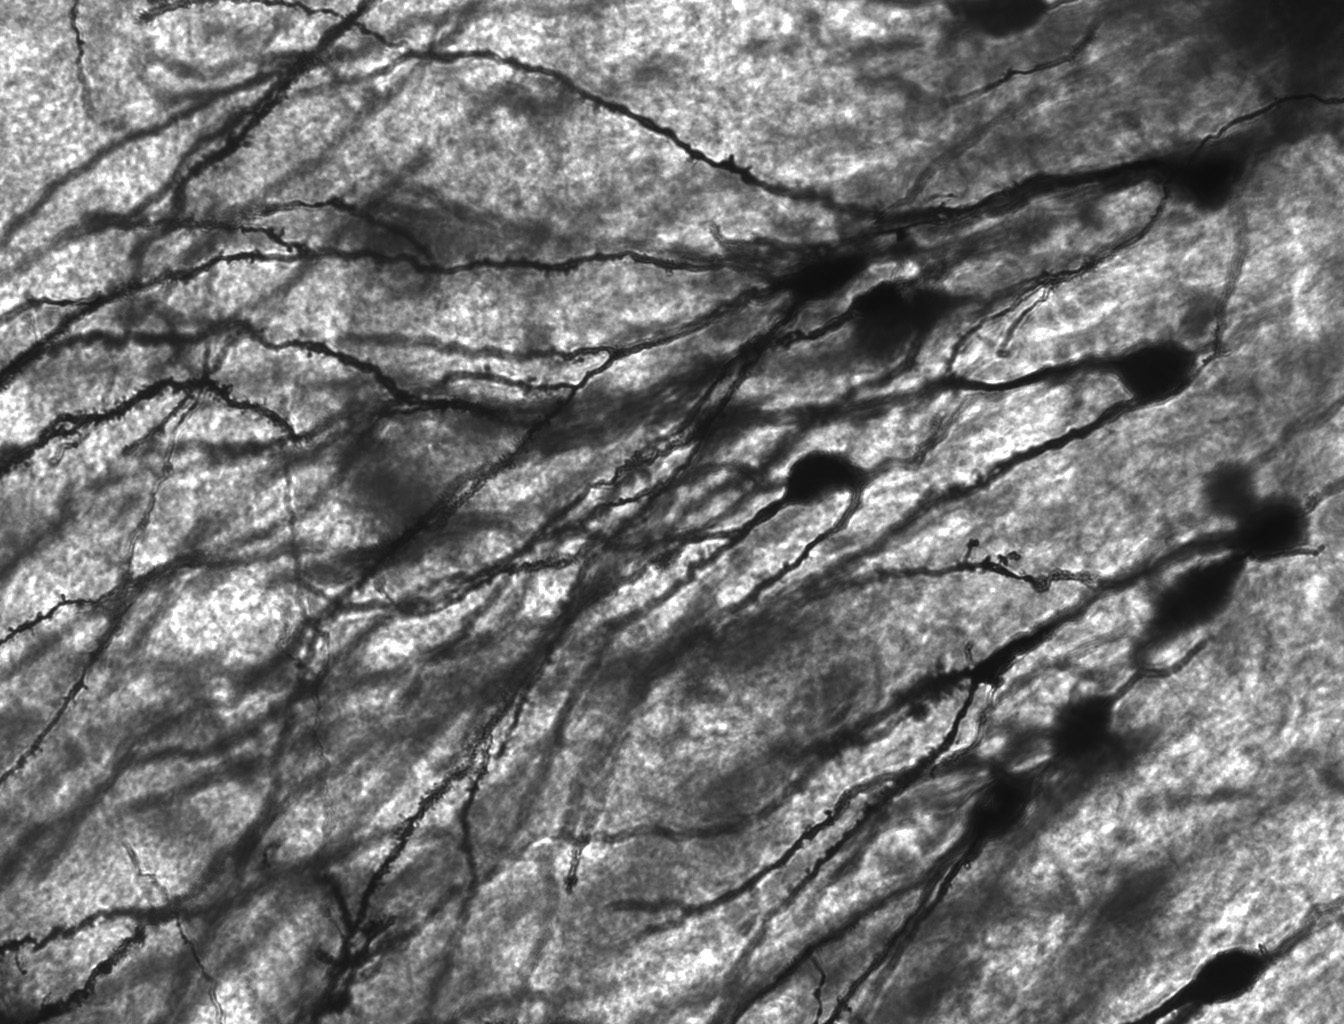
\includegraphics[width=0.8\linewidth]{images/Gyrus_Dentatus_40x}}
%  \caption{Neurons in the dentate gyrus of an epilepsy patient.}
%\end{figure}

\begin{Figure}
 \centering
 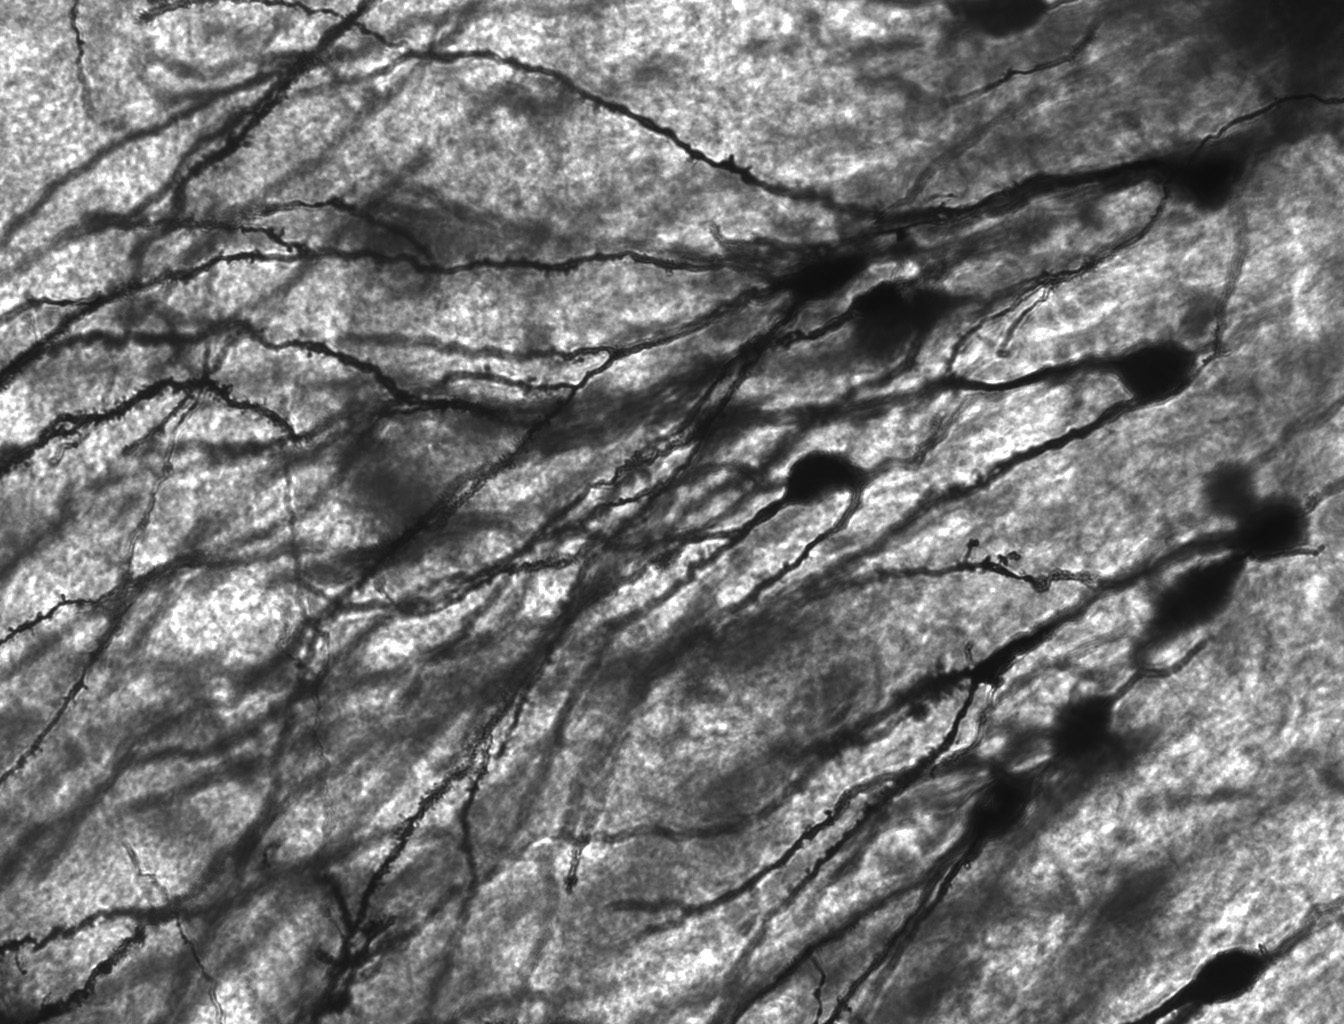
\includegraphics[width=0.8\linewidth]{images/Gyrus_Dentatus_40x}
 \captionsetup{width=0.8\linewidth, font=small}
 \captionof{figure}{Neurons in the dentate gyrus of an epilepsy patient.}
\end{Figure}

While obviously interesting within the fields of biology or psychology, this structure has shown 
to be enourmously interesting in the field of computation, as one can in fact model this very 
thing and use it to make predictions based on prior observations, for example in regards to the 
aforementioned structures of proteins folding.

Analogously, or rather, digitally, we can use this model to construct an \textit{artificial 
neural network}.
These set themselves apart from biological neural networks in a couple of ways: most urgently in that while neurons in biological neural networks are connected to each other via synapses, so that each neuron has an either inhibitory or activating effect on whether or not a connected neuron 'fires', in artificial neural networks neurons are connected by \textit{edges}, each with an associated \textit{weight}, allowing the artificial networks to leave the discrete domain and enter the continuous.

\subsubsection{Basics}
An artificial neural network is a specific instantiation of a \textit{multi-layer perceptron}.
A multi-layer perceptron in turn is a system of nodes arranged into layers and each receiving their value from the value of the nodes in the layer before them (adjusted by some weight) in combination with a bias (a scalar) and an activation function of some sort. \\
In this way the first layer will be called the \textit{input layer}, the last layer the \textit{output layer} and all layers in between \textit{hidden layers}. \\
In the case of neural networks, the nodes in the system are referred to as neurons.
Thus, if one was to describe it more precisely, the value $z_i$ of neuron layer \textit{i} with \textit{d} number of neurons in it, given the matrix of sets of weights \textit{w} (the biases being the very first row) and the activation function $h()$ can be expressed as follows:
\[
z_i = h\left(\sum_{j=0}^d w_{ij}\cdot z_{i-1} + w_{i0}\right)
\]
Such a model is useful for calculating continuous values as well as for classification purposes. A common example of the latter is the MNIST data set of hand-written digits in 28x28 pixel greyscale images. In this case the light intensity of the 784 ($28^2$) pixels could fittingly be the input layer, while a layer consisting of 10 nodes (corresponding to digits 0 through 9) could be the output layer, such that the system could be used to predict which digit is written in a given image.
%\begin{figure}[h]
%  \centering
%  \frame{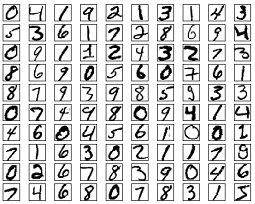
\includegraphics[width=0.7\linewidth]{images/mnist}}
%  \caption{Handwritten digits in the MNIST data set.}
%\end{figure}

\begin{Figure}
 \centering
 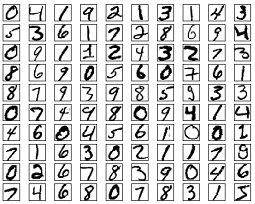
\includegraphics[width=0.7\linewidth]{images/mnist}
 \captionsetup{width=0.8\linewidth, font=small}
 \captionof{figure}{Handwritten digits in the MNIST data set.}
\end{Figure}

A common implementation of a neural network to perform this task is to have a single hidden layer of 800 nodes, however the most successful implementations in regards to the MNIST data set have been made with \textit{convolutional neural networks}, but we shall return to these later.

\subsubsection{Training}
Simply having defined the system of the neural network as above (denoted $f_{NN}$) naturally does not give us a reliable method for classifying, as the accuracy of the prediction inherently depends on the correctness of the weights and biases of the system (denoted $\Theta$), which must be initialized with random values. \\
Enter a rather nifty idea named \textit{backpropagation}. Having a set of predicted values ($\hat{y}$) for a data set (\textit{x}) along with the observed correct values (\textit{y}), one can establish a \textit{loss} by applying a loss function (that we shall elaborate on later), but which can be as straightforward as a root mean square error. We shall denote this loss function $l(\hat{y},y)$, so that the  total loss of the system when applied to data set \textit{x} is $l(f_{NN}(\Theta, x), \hat{y})$.\\
Now backpropagation refers to the practice of essentially taking the derivative of the loss function in regards to the matrix of weights and biases, thereby calculating a \textit{gradient} $\nabla{l(f_{NN}(\Theta, x), \hat{y})}$ of these values with respect to the accuracy of the system, and then adjusting the weights and biases by the gradient multiplied by a learning rate scalar.\\
In laymans terms, by doing this one gets a matrix of 'change your weights by this and that much in this and that direction to increase prediction accuracy'.
%
%\begin{tikzpicture}[line cap=round,line join=round,>=triangle 45,x=0.4cm,y=0.4cm]
%\clip(-3.84,0.01) rectangle (18.8,18.55);
%\draw [line width=1pt,fill=ffqqqq,fill opacity=1] (2,7) circle (0.4cm);
%\draw [line width=1pt,fill=ffqqqq,fill opacity=1] (2,10) circle (0.4cm);
%\draw [line width=1pt,fill=qqffqq,fill opacity=1] (7,4) circle (0.4cm);
%\draw [line width=1pt,fill=qqffqq,fill opacity=1] (7,7) circle (0.4cm);
%\draw [line width=1pt,fill=qqffqq,fill opacity=1] (7,10) circle (0.4cm);
%\draw [line width=1pt,fill=qqffqq,fill opacity=1] (7,13) circle (0.4cm);
%\draw [line width=1pt,fill=qqttcc,fill opacity=1] (12,10) circle (0.4cm);
%\draw [line width=1pt,fill=qqttcc,fill opacity=1] (12,7) circle (0.4cm);
%\draw [line width=1pt] (3,10)-- (6,13);
%\draw [line width=1pt] (3,10)-- (6,10);
%\draw [line width=1pt] (3,10)-- (6,7);
%\draw [line width=1pt] (3,10)-- (6,4);
%\draw [line width=1pt] (3,7)-- (6,13);
%\draw [line width=1pt] (3,7)-- (6,10);
%\draw [line width=1pt] (3,7)-- (6,7);
%\draw [line width=1pt] (3,7)-- (6,4);
%\draw [line width=1pt] (8,13)-- (11,10);
%\draw [line width=1pt] (8,10)-- (11,10);
%\draw [line width=1pt] (8,7)-- (11,10);
%\draw [line width=1pt] (8,4)-- (11,10);
%\draw [line width=1pt] (8,4)-- (11,7);
%\draw [line width=1pt] (11,7)-- (8,7);
%\draw [line width=1pt] (8,10)-- (11,7);
%\draw [line width=1pt] (11,7)-- (8,13);
%\end{tikzpicture}

\subsubsection{Convolutional neural networks}
Before talking about convolutional neural networks, we have to specify what a convolution is. Again the MNIST data set serves as an obvious example.\\
One can understand each of the images in the data set as a matrix of $28\times28$ values in the range of 0 - 255. The word convolution comes from the latin convolvere, meaning to roll or to coil and still has a similar meaning in english today. In math convolution is an operation where, for two functions f(x) and g(x), one is shifted across the other, which result in a third function h(x) that express the the intersection of the two functions. As such h(x) explains how the shape of one of the functions is changed by the other. 
However the more practical explanation in the case of our thesis, is that it is the resulting matrix of the product of a matrix and a filter. For example if one has the matrix $a$ and the filter $f$:
\[
a = \begin{bmatrix}
       2 & 3 & 4           \\[0.3em]
       1 & 2 & 3 \\[0.3em]
       0 & 1 & 2
     \end{bmatrix}
\hspace*{1cm}
f = \begin{bmatrix}
       0 & 1 \\[0.3em]
       1 & 0        
     \end{bmatrix}     
\]

the resulting output of convolving $f$ over $a$ would be:

\[
\begin{bmatrix}
       4 & 6 \\[0.3em]
       2 & 4        
     \end{bmatrix}     
\]

where convolving works as follows:
\[
\begin{bmatrix}
       \textcolor{red}2 & \textcolor{red}3 & 4           \\[0.3em]
       \textcolor{red}1 & \textcolor{red}2 & 3 \\[0.3em]
       0 & 1 & 2
     \end{bmatrix}
\hspace*{0.5cm}
*
\hspace*{0.5cm}
\begin{bmatrix}
       0 & 1 \\[0.3em]
       1 & 0        
     \end{bmatrix}     
\hspace*{1cm}
 = \begin{bmatrix}
       \textcolor{red}4 &  \\[0.3em]
         &         
     \end{bmatrix}
\]

\[
\begin{bmatrix}
       2 & \textcolor{red}3 & \textcolor{red}4           \\[0.3em]
       1 & \textcolor{red}2 & \textcolor{red}3 \\[0.3em]
       0 & 1 & 2
     \end{bmatrix}
\hspace*{0.5cm}
*
\hspace*{0.5cm}
\begin{bmatrix}
       0 & 1 \\[0.3em]
       1 & 0        
     \end{bmatrix}     
\hspace*{1cm}
 = \begin{bmatrix}
       4 & \textcolor{red}6 \\[0.3em]
         &         
     \end{bmatrix}
\]
\[
\begin{bmatrix}
       2 & 3 & 4           \\[0.3em]
       \textcolor{red}1 & \textcolor{red}2 & 3 \\[0.3em]
       \textcolor{red}0 & \textcolor{red}1 & 2
     \end{bmatrix}
\hspace*{0.5cm}
*
\hspace*{0.5cm}
\begin{bmatrix}
       0 & 1 \\[0.3em]
       1 & 0        
     \end{bmatrix}     
\hspace*{1cm}
 = \begin{bmatrix}
       4 & 6 \\[0.3em]
       \textcolor{red}2 &         
     \end{bmatrix}
\]
\[
\begin{bmatrix}
       2 & 3 & 4           \\[0.3em]
       1 & \textcolor{red}2 & \textcolor{red}3 \\[0.3em]
       0 & \textcolor{red}1 & \textcolor{red}2
     \end{bmatrix}
\hspace*{0.5cm}
*
\hspace*{0.5cm}
\begin{bmatrix}
       0 & 1 \\[0.3em]
       1 & 0        
     \end{bmatrix}     
\hspace*{1cm}
 = \begin{bmatrix}
       4 & 6 \\[0.3em]
       2 & \textcolor{red}4        
     \end{bmatrix}
\]

As can be seen on the above example there is a couple of things to consider in regard to convolution. First is, when done as above, the size of the input matrix is different than the output matrix, due to the filter size. This filter is also known as the kernel, so when kernel size is mentioned, it is the size of the filter used for convolution. If it had been important to have an output matrix of the same size as the input, a way to achieve this would be using zero padding. Zero padding would be adding zeros to the input matrix so it became a 4x4 matrix, so when when shifting the kernel across, the output would be the original 3x3. Of course the amount of padding needed also depends on the kernel size. Had the kernel been size 3x3, for the output matrix to be 3x3, it would have been necessary to pad zeros all around the original input matrix so it would be a 5x5 before convolution. Another parameter worth considering when doing convolution is what is called stride. In the above example we saw how we started in the upper left corner of the matrix, then moved the kernel one step to the right, then down to the left and then to the right again. This was a stride of size 1. If the matrix had been a 6x6, and our kernel still was a size 2x2, we would still have started in the upper left corner, then moved it one step to the right, then another, and then another, until the right side of the kernel had shiftet to align with the right side of the matrix. Then it would be moved on step down and all the way to the left again, and then one step at a time to the right once more. Now, if it had been a stride of size 2 instead in a 6x6 and a kernel size 2x2, it would start in the upper left, then move 2 to the right instead of one, but otherwise follow the same pattern of movement. This has a couple of effects. One of course is how the kernel is applied to the matrix. Another is the output will be down sampled, kind of like we saw when the input matrix was not zero padded. 



\subsubsection{Multitask learning}

The concept of multitask learning is both simple and ingenious. It's foundation is that, when training a neural network to predict a certain task given a set of parameters, by training it to predict another or maybe several tasks instead of a single one, each individual prediction will reach a better accuracy. The idea behind it is to use domain-specific information in the training signals of related tasks, to improve the generalization of a model. By training a model to have good predictions on more than one task, data dependent noise related to one task will then be identified easier as something to be ignored and thereby the general accuracy will increase. Furthermore when having a limited dataset with a lot of noise, the model will, by having several tasks to predict, have help in focusing the attention on the relevant features that lead to correct predictions, and ignoring data specific features that might lead to overfitting. 

\subsection{Prior research in this field}

As protein secundary structure prediction is an important field for several scientific fields with ongoing research and real world application, it follows that there exists a lot of papers on the subject. We have used 4 articles extensively for this thesis. As such we wish to shortly present them and the content they have brought to this thesis. 
The main paper and starting point for our thesis was Zhou and Troyanskaya’s “Deep Supervised and Convolutional Generative Stochastic Network for Protein Secondary Structure prediction”. The dataset we have been using for training our own network was the one they made for this proceeding. Besides presenting the dataset and giving a deeper understanding of it, the paper gave other insights as well. Though a lot of the methods and architecture they present are outside the scope of this thesis, Zhou and Troyanskaya’s paper gives a good understanding of what a neural network is and further gave an idea about what we could expect accuracy-wise when trying to predict protein secondary structures. 
The next paper we used were Qi et al.’s “A unified Multitask Architecture for Predicting Local Protein Properties”. As Zhou and Troyanskaya had used the method from this paper to discretize solvent accessibility scores to absolute and releative solvent accessibility, it brought to the table further understanding of our dataset. Furthermore the paper is about using multitask learning for secondary structure prediction, and as the final goal of this thesis is to understand and implement a convolutional neural network using multitask learning, a lot of inspiration was drawn from this paper. Lastly this paper gives a good understanding and basic introduction to the biological background of proteins and the features of the protein one can try to predict. 
Our two last research papers are Wang et al.’s “Protein Secondary Structure Prediction Using Deep Convolutional Neural Fields” and Ruder’s ”An Overview of Multi-Task Learning in Deep Neural Networks”.  As Wang et al. also are predicting secondary structure using convolution we took inspiration from here as well, especially when starting out looking to optimize our hyperparameters. Wang et al. also gave us and even better and more updated understanding of expectancy for accuracy as they achieve ~73 \% accuracy on a CullPDB dataset. Ruder being our last main paper, gives a good introduction to the methodology of multitask learning and the ideas behind. As such much of our methodology concerning multitask learning will come from his paper.











